\chapter{ 介绍
  % Introduction
}

This document describes the RISC-V privileged architecture, which
covers all aspects of RISC-V systems beyond the unprivileged ISA,
including privileged instructions as well as additional functionality
required for running operating systems and attaching external devices.

本文描述了RISC-V特权指令架构,其覆盖了在非特权ISA基础上的RISC-V系统的
各个方面,包括特权指令以及运行操作系统和其它外设需要的额外功能

\begin{commentary}
Commentary on our design decisions is formatted as in this paragraph,
and can be skipped if the reader is only interested in the
specification itself.

如果读者只关心规范本身,本段落的注释可以忽略。
\end{commentary}

\begin{commentary}
We briefly note that the entire privileged-level design described in
this document could be replaced with an entirely different
privileged-level design without changing the unprivileged ISA, and
possibly without even changing the ABI.  In particular, this
privileged specification was designed to run existing popular
operating systems, and so embodies the conventional level-based
protection model.  Alternate privileged specifications could embody
other more flexible protection-domain models.  For simplicity of
expression, the text is written as if this was the only possible
privileged architecture.

在不改变非特权指令集,甚至不改变ABI的情况下,本文描述的特权层级
设计可以完全用不同的特权层级设计取代。这种特权规范设计可以与当前
流行的操作系统相适应,体现了传统传统的基于层级的保护模型。另外,
特权规范可以体现其它更多的基于域保护的模型。为简洁起见,本文以
一种可能的特权架构进行撰写。
\end{commentary}

\section{RISC-V Privileged Software Stack Terminology}

This section describes the terminology we use to describe components
of the wide range of possible privileged software stacks for RISC-V.

本节对RISC-V的特权软件栈涉及的相关专业名词进行描述。

Figure~\ref{fig:privimps} shows some of the possible software stacks
that can be supported by the RISC-V architecture.  The left-hand side
shows a simple system that supports only a single application running
on an application execution environment (AEE).  The application is
coded to run with a particular application binary interface (ABI).
The ABI includes the supported user-level ISA plus a set of ABI calls to
interact with the AEE.  The ABI hides details of the AEE from the
application to allow greater flexibility in implementing the AEE.  The
same ABI could be implemented natively on multiple different host OSs,
or could be supported by a user-mode emulation environment running on
a machine with a different native ISA.

图~\ref{fig:privimps}展示了支持RISC-V架构的可能软件栈。左图显示一个
简单的系统,这个系统只支持在应用执行环境(AEE)里面运行单一的程序。
应用程序执行时与一个特殊的应用二进制接口(ABI)一起运行。ABI包括支持
的用户层级ISA,和一系列与AIEE交互的ABI调用。从应用程序的角度看,ABI隐藏了
AEE的细节,这对于AEE的实现提供了更多的弹性。同样的ABI可能被不同的宿主
操作系统本地化实现,或者被不同不同ISA的机器运行的用户态模拟环境支持。

\begin{figure}[th]
\centering
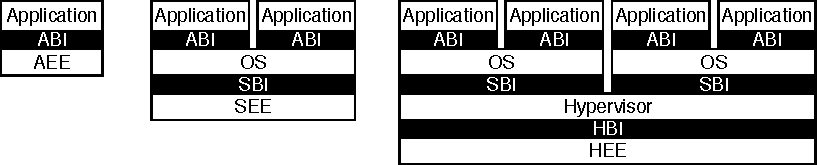
\includegraphics[width=\textwidth]{figs/privimps.pdf}
\caption{Different implementation stacks supporting various forms of
  privileged execution.}
\label{fig:privimps}
\end{figure}

\begin{commentary}
Our graphical convention represents abstract interfaces using black
boxes with white text, to separate them from concrete instances of
components implementing the interfaces.

我们通常用黑框白字表示抽象接口,将其与实现接口的具体实例区别。
\end{commentary}

The middle configuration shows a conventional operating system (OS)
that can support multiprogrammed execution of multiple
applications. Each application communicates over an ABI with the OS,
which provides the AEE.  Just as applications interface with an AEE
via an ABI, RISC-V operating systems interface with a supervisor
execution environment (SEE) via a supervisor binary interface (SBI).
An SBI comprises the user-level and supervisor-level ISA together with
a set of SBI function calls.  Using a single SBI across all SEE
implementations allows a single OS binary image to run on any SEE.
The SEE can be a simple boot loader and BIOS-style IO system in a
low-end hardware platform, or a hypervisor-provided virtual machine in
a high-end server, or a thin translation layer over a host operating
system in an architecture simulation environment.

中间的配置显示了一个支持多程序执行的操作系统。每个应用与OS的ABI交互,
OS为其提供AEE。RISC-V操作系统与特权执行环境(SEE)通过一个特权二进制
接口(SBI)进行交互。SBI由用户级和特权级ISA以及一套SBI函数调用组成。通过
一个所有SEE实现都支持的SBI,一个操作系统影响可以运行在任意的SEE上。
SEE可能是底层硬件平台的一个简单的启动加载和BIOS风格的IO系统,也可能是一个
高端服务器里面的超级虚拟机,或者是一个体系架构模拟环境里的宿主操作系统上的
一个瘦中继层。
\begin{commentary}
Most supervisor-level ISA definitions do not separate the SBI from the
execution environment and/or the hardware platform, complicating
virtualization and bring-up of new hardware platforms.

大部分超级ISA定义不会将SBI与可执行环境或/和硬件平台分开(那样将会使虚拟化复杂
并产生新的硬件平台)
\end{commentary}

The rightmost configuration shows a virtual machine monitor
configuration where multiple multiprogrammed OSs are supported by a
single hypervisor.  Each OS communicates via an SBI with the
hypervisor, which provides the SEE.  The hypervisor communicates with
the hypervisor execution environment (HEE) using a hypervisor binary
interface (HBI), to isolate the hypervisor from details of the
hardware platform.

最右边的配置展示了一个虚拟机监视器的配置,在其中,一个单一的超级进程支持
多个多进程操作系统。每个操作系统通过SBI与提供SEE的超级管理进程进行交互。
超级管理进程以HBI接口的形式与HEE进行交互,从而将超级管理者与具体的硬件细节解耦。

\begin{commentary}
The ABI, SBI, and HBI are still a work-in-progress, but we are now
prioritizing support for Type-2 hypervisors where the SBI is provided
recursively by an S-mode OS.

ABI、SBI、和HBI规范依然在演进,我们优先支持第二种类型的超级进程,这种模式里面,
SBI由安全模式操作系统递归提供支持
\end{commentary}

Hardware implementations of the RISC-V ISA will generally require
additional features beyond the privileged ISA to support the various
execution environments (AEE, SEE, or HEE).

为了支持不同的执行环境(AEE,SEE,HEE),RISC-V ISA的硬件实现需要
在特权ISA的基础上增加额外的特征。

\section{Privilege Levels}

At any time, a RISC-V hardware thread ({\em hart}) is running at some
privilege level encoded as a mode in one or more CSRs (control and
status registers).  Three RISC-V privilege levels are currently defined
as shown in Table~\ref{privlevels}.

在任意时刻,一个RISC-V线程运行在某个特权层级(以一个或多个CSR进行编码)。
表~\ref{privlevels}定义了三种RISC-V特权层级。

\begin{table*}[h!]
\begin{center}
\begin{tabular}{|c|c|c|c|}
  \hline
   Level & Encoding & Name      & Abbreviation \\ \hline  
   0     & \tt 00   & User/Application & U     \\ 
   1     & \tt 01   & Supervisor & S           \\ 
   2     & \tt 10   & {\em Reserved} &            \\ 
   3     & \tt 11   & Machine    & M           \\ 
  \hline
 \end{tabular}
\end{center}
\caption{RISC-V privilege levels.}
\label{privlevels}
\end{table*}

Privilege levels are used to provide protection between different
components of the software stack, and attempts to perform operations
not permitted by the current privilege mode will cause an exception to
be raised.  These exceptions will normally cause traps into an
underlying execution environment.

特权层级为软件栈的不同组建提供保护,在当前特权模式执行不允许的操作将
导致抛出异常。这种异常导致陷入底层的执行环境。

\begin{commentary}
In the description, we try to separate the privilege level for which
code is written, from the privilege mode in which it runs, although
the two are often tied.  For example, a supervisor-level operating
system can run in supervisor-mode on a system with three privilege
modes, but can also run in user-mode under a classic virtual machine
monitor on systems with two or more privilege modes.  In both cases,
the same supervisor-level operating system binary code can be used,
coded to a supervisor-level SBI and hence expecting to be able to use
supervisor-level privileged instructions and CSRs.  When running a
guest OS in user mode, all supervisor-level actions will be trapped
and emulated by the SEE running in the higher-privilege level.

在本文的描述中,我们试图将运行代码的特权层级与其运行的特权模式相区分,
虽然二者通常紧密联系在一起。例如,一个超级层级操作系统可以三种特权
模式运行在系统的超级模式,它也可以在经典虚拟机下以用户模式运行
在具有两个或多个特权模式的系统上运行。在这两种情况下,同一个超级层级操作系统
二进制代码可以被编码为超级层级SBI,从而能够使用超级层级特权指令和相应的CSR。
当在用户模式运行宾客操作系统是,所有的超级层级行为被捕获并被更高特权层级运行
的SEE模拟。
\end{commentary}

The machine level has the highest privileges and is the only mandatory
privilege level for a RISC-V hardware platform.  Code run in
machine-mode (M-mode) is usually inherently trusted, as it has
low-level access to the machine implementation.  M-mode can be used to
manage secure execution environments on RISC-V.  User-mode (U-mode)
and supervisor-mode (S-mode) are intended for conventional application
and operating system usage respectively.

机器层级拥有最高的特权,它是RISC-V硬件平台的唯一强制性特权层级。在机器模式下运行
的代码被认为是天然可信的,它对计算机的底层硬件直接访问。机器模式用于管理RISC-V的
安全可执行环境。用户模式和监控模式分别适用于传统的应用程序和操作系统。

Each privilege level has a core set of privileged ISA extensions with optional
extensions and variants.  For example, machine-mode supports an optional
standard extension for memory protection.  Also, supervisor mode can be
extended to support Type-2 hypervisor execution as described in
Chapter~\ref{hypervisor}.

每一个特权层级拥有一系列核心特权ISA及其可选的扩展和变量。例如,机器模式针对内存保护
支持可选的辨准扩展。此外,监控模式可以扩展以支持 2 类虚拟机管理程序执行,如
📈~\ref{hypervisor}中所述。


Implementations might provide anywhere from 1 to 3 privilege modes
trading off reduced isolation for lower implementation cost, as shown
in Table~\ref{privcombs}.

具体实现可以提供1到3中权限模式,以降低底层实现之间的解耦成本。如表~\ref{privcombs}所示。
in table~ref{privcombs}.


\begin{table*}[h!]
\begin{center}
\begin{tabular}{|c|l|l|}
  \hline
   Number of levels &  Supported Modes & Intended Usage \\ \hline  
   1     & M          & Simple embedded systems \\ 
   2     & M, U       & Secure embedded systems \\ 
   3     & M, S, U    & Systems running Unix-like operating systems\\ 
  \hline
 \end{tabular}
\end{center}
\caption{Supported combinations of privilege modes.}
\label{privcombs}
\end{table*}

All hardware implementations must provide M-mode, as this is the only
mode that has unfettered access to the whole machine.  The simplest
RISC-V implementations may provide only M-mode, though this will
provide no protection against incorrect or malicious application code.

所有对了硬件实现必须提供机器模式,因为它是唯一的
可以不受限制地访问整个机器的模式。最简单的RISC-V实现可以只提供机器模式,
但是这样就会导致错误访问或恶意代码保护的确实。

\begin{commentary}
  The lock feature of the optional PMP facility can provide some
  limited protection even with only M-mode implemented.
  
  可选PMP的锁特性能为仅仅提供机器模式的实现提供有限的保护。
\end{commentary}

Many RISC-V implementations will also support at least user mode
(U-mode) to protect the rest of the system from application code.
Supervisor mode (S-mode) can be added to provide isolation between a
supervisor-level operating system and the SEE.

许多RISC-V在机器模式的基础上至少支持用户模式,用于保护系统。加入监控
模式可以将将监控层级操作系统和SEE隔离。

A hart normally runs application code in U-mode until some trap (e.g.,
a supervisor call or a timer interrupt) forces a switch to a trap
handler, which usually runs in a more privileged mode. The hart will
then execute the trap handler, which will eventually resume execution
at or after the original trapped instruction in U-mode.  Traps that
increase privilege level are termed {\em vertical} traps, while traps
that remain at the same privilege level are termed {\em horizontal}
traps.  The RISC-V privileged architecture provides flexible routing
of traps to different privilege layers.

在hart里,应用代码通常运行在用户模式下,当捕获到某个陷阱时切换到特权级别更高的陷阱处理程序。
hart这个时候会运行陷阱处理程序,在陷阱处理程序执行完之后,它将返回到用户模式下继续执行。
增加特权层级的陷阱称之为{\em 垂直} 陷阱,保持原有特权层级的陷阱称之为{\em 水平}陷阱。RISC-V
特权架构为不同的特权成提供具有弹性路由的陷阱。

\begin{commentary}
Horizontal traps can be implemented as vertical traps that
return control to a horizontal trap handler in the less-privileged mode.

水平陷阱也可以通过在低特权即模式下返回一个水平陷阱的控制去实现垂直陷阱。
\end{commentary}

\section{Debug Mode}

Implementations may also include a debug mode to support off-chip
debugging and/or manufacturing test.  Debug mode (D-mode) can be
considered an additional privilege mode, with even more access than
M-mode. The separate debug specification proposal describes operation
of a RISC-V hart in debug mode.  Debug mode reserves a few CSR
addresses that are only accessible in D-mode, and may also reserve
some portions of the physical address space on a platform.

实现还可能包括支持片外的调试模式调试和/或制造测试。 
调试模式(D 模式)可以认为是一种额外的特权模式,它具有比机器模式更多的访问。
单独的调试规范提案描述了调试模式下的RISC-V hart操作。 调试模式保留一些只能在
D模式下访问的CSR地址,也保留了物理地址空间上的某个部分。

